\documentclass{article}

\usepackage{listings}
\usepackage{graphicx}

\title{How to create a \LaTeX~document from a Maxima script}
\author{Richel Bilderbeek}
\date{\today}

\begin{document}

\maketitle

\begin{abstract}
This article is created within the CAS program Maxima
and shows (1) algebraic differentiation (2) plotting, and (3) listings.
This article is self-containing: it can be recreated from the listings it contains.
The article itself is intended to be of
publishable quality, having (1) an abstract (2) a bibliography.
\end{abstract}

\section{Introduction}

\LaTeX~is commonly used for writing publishable scientific articles\cite{gaudeul2006}.
Algebraic manipulations can be done by a CAS, for example Maxima, Maple or Mathematica.
Maxima is the only free and open-source program, and it is the oldest free and open-source computer algebra system, with development started in 1967 (as Macsyma) or 1982 (as MAXIMA).
This article is an example of writing a \LaTeX~ article within Maxima

\section{Materials and methods}

A script executes the process from Maxima file to \LaTeX-formatted document in two steps.
The first step executes the Maxima script to create a \LaTeX~(.tex) file.
The second step converts the \LaTeX~file to Portable Document Format (.pdf).
The script does not require user intervention.

The Maxima script consists out of two parts:
algebraic manipulations and \LaTeX~output

The algebraic manipulations demonstrated are: 
(1) defining a function
(2) calculate its derivative and,
(3) plot this derivative.

The second part uses these algebraic results to create a \LaTeX~(.tex) file.
It creates an article displaying the formula's, the single plot in
the Results section.
In the Appendix, it shows: 
(1) the bash script to create a PDF from the Maxima script
(2) the Maxima script
(3) the generated \LaTeX~code

\section{Results}

Equation $f(x)$ used:

$$f\left(x\right)=1.0 \times 10^{-4}\,x^4-0.002\,x^3+0.03\,x^2-0.4\,x
 +1$$

Equation $g(x)$ is the derivative of $f(x)$ with respect to $x$:

$$g\left(x\right)=4.0 \times 10^{-4}\,x^3-0.006\,x^2+0.06\,x-0.4$$

Equation $h(x,y) = f(x) + g(y)$, which equates to:

$$h\left(x , y\right)=4.0 \times 10^{-4}\,y^3-0.006\,y^2+0.06\,y+
 1.0 \times 10^{-4}\,x^4-0.002\,x^3+0.03\,x^2-0.4\,x+0.6$$

Plotting $g(x)$:

\fbox{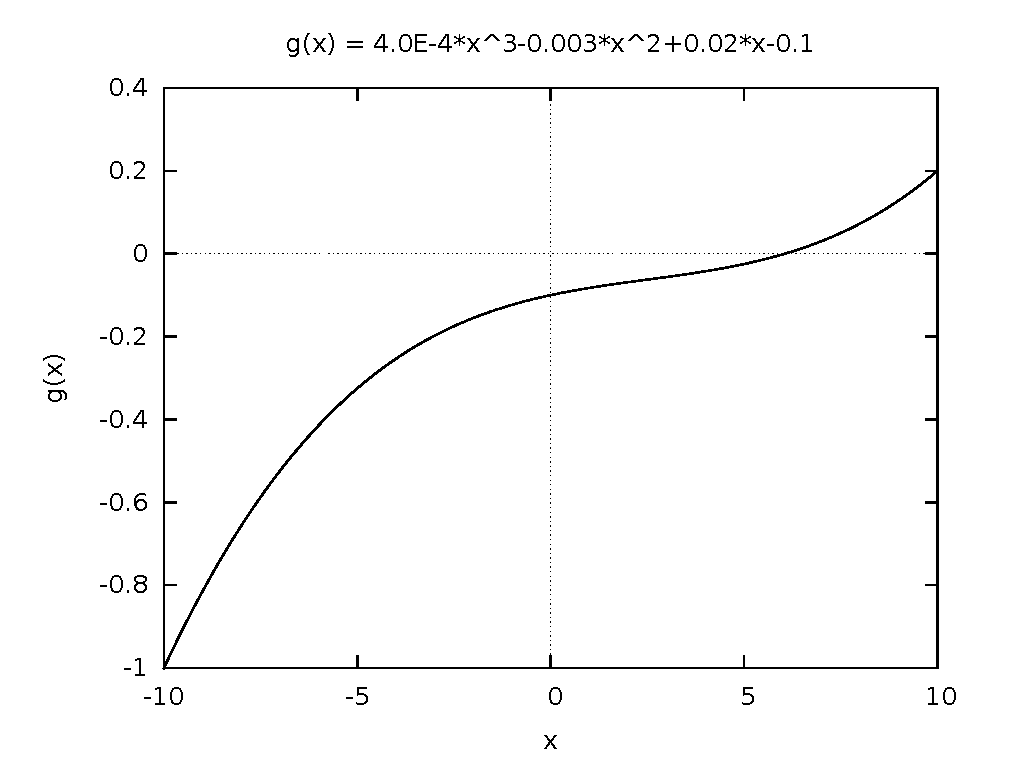
\includegraphics[scale=0.8]{/home/richel/GitHubs/Maxima/create_tex_article_output_plot2d.pdf}}
Plotting $h(x,y)$:

\fbox{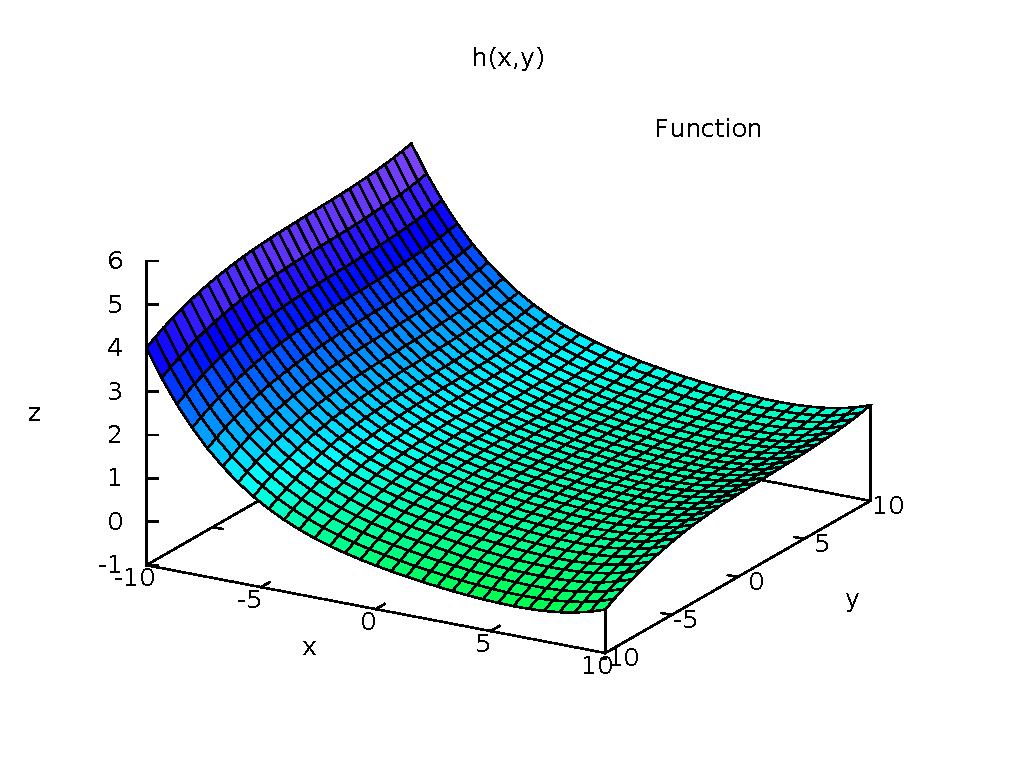
\includegraphics[scale=0.8]{/home/richel/GitHubs/Maxima/create_tex_article_output_plot3d.pdf}}

\section{Discussion}

Writing \LaTeX~within Maxima can be done, but it is a bit cumbersome:
Maxima does not know \LaTeX~syntax and just creates contextless strings,
which might not be compilable by \LaTeX.
However, because the script does create a .tex file,
this file can be inspected easily with a \LaTeX~tool like texmaker.

\begin{thebibliography}{9}

\bibitem{gaudeul2006}
  Gaudeul, A.
  2006
  Do Open Source Developers Respond to Competition?: The (La)TeX Case Study.
  Available at SSRN: http://ssrn.com/abstract=908946 or http://dx.doi.org/10.2139/ssrn.908946
\end{thebibliography}

\appendix

\section{Script file}

\lstinputlisting[language=C++,showstringspaces=false,breaklines=true,frame=single]{create_tex_article.sh}

\section{Maxima file}

\lstinputlisting[language=C++,showstringspaces=false,breaklines=true,frame=single]{create_tex_article.txt}

\section{\LaTeX~file}

\lstinputlisting[language=tex,showstringspaces=false,breaklines=true,frame=single]{create_tex_article_output.tex}

\end{document}
